\documentclass[a4,12pt]{article}
	\usepackage[UTF8]{ctex}
	\usepackage{datetime2}% to use \DTMnow
	\usepackage{indentfirst}
		\setlength{\parskip}{5pt}% spacing between paragraphs
		\setlength{\parindent}{20pt}% indentation
	\usepackage{geometry}
		\geometry{tmargin=8mm,bmargin=15mm,lmargin=8mm,rmargin=8mm}
	\usepackage{enumitem}
	\usepackage{amsmath}
	\usepackage{amssymb}% use mathcal, etc.
	\usepackage{mathtools}
	\usepackage{physics}
	\usepackage{tabu}
	\usepackage{tikz}
		\usetikzlibrary{arrows.meta,calc,decorations.markings,math,arrows.meta,patterns,angles,quotes,decorations.pathreplacing}

% self-defined commands always begin with UPPERCASE LETTER
	\newenvironment{LatinModern}{\fontfamily{lmr}\selectfont}{\par}% Latin Modern
	\DeclareTextFontCommand{\textmyfont}{\LatinModern}
	\newcommand{\Curs}[1]{\emph{\LatinModern{#1}}}
	\newcounter{Problem}
	\newcommand{\Problem}[1]{
		\vspace*{10pt}
		\stepcounter{Problem}
		\label{Problem \arabic{Problem}}
		\noindent\arabic{Problem}.\emph{~#1}
	}
	\newcommand{\Qed}{\hfill\ensuremath{\square}}

% useful symbols
	\def\Tick{\ding{51}}
	\newcommand{\rectangle}{{
		\ooalign{$\sqsubset\mkern3mu$\cr$\mkern3mu\sqsupset$\cr}
	}}

\begin{document}

% Title
	\title{
		\vspace*{-50pt}
		\Large{\textbf{太平华联中学数学竞赛题解}\vspace*{-10pt}}\\
	}
	\author{作者:郑其恩 Fanurs\vspace*{-30pt}}
	\date{最后编译时间:\DTMnow (美东)}
	\maketitle
	\vspace*{-25pt}

\setcounter{Problem}{0}
\Problem{
	$5^{20}\times4^{17}$这个数有几位数?
	}

	这种题型的技巧在于,从数字中抽取出$5^n\times2^m$形式的因数,而后利用$5^k\times2^k = 10^k$的特性把数字以科学计数法表达。
	\[\begin{aligned}
		\mbox{原数}
		&= 5^{20}\times4^{17} \\
		&= 5^{20}\times2^{2\times17} \\
		&= (5^{20}\times2^{20})\times2^{34-20} \\
		&= 2^{14}\times10^{20} \\
		&= 16384\times10^{20} \ \mbox{。}
		\end{aligned}
	\]
	因此,这个数一共有$5+20=25$位数。
	\Qed
	\vspace*{30pt}

	\noindent 点评:
	\begin{enumerate}[label=(\alph*)]
		\item $2^n$是竞赛中常出现的数,鼓励参赛同学至少熟记$n=10$以内的数。
	\end{enumerate}

\pagebreak
\Problem{
	已知一数列$a_1, a_2, a_3, \ldots$满足以下条件:
	\begin{center}对于所有的$n\ge1$,$a_1+a_2+a_3+\cdots+a_n=n^3$。\end{center}
	求$a_{100}$的最后三位数。
	}

	根据题目,可列出
	\[ \begin{aligned}
		a_1+a_2+\cdots+a_{99} &= 99^3 \\
		a_1+a_2+\cdots+a_{99}+a_{100} &= 100^3
		\end{aligned}
	\]
	因此,
	\[ \begin{aligned}
			a_{100}
			&= 100^3 - 99^3 \\
			&= 100^3 - (100-1)^3 \\
			&= 100^3 - (100^3 - 3\times100^2 + 3\times100 - 1) \\
			&= 30000 - 300 + 1 \\
			&= 29701 \ \mbox{。}
		\end{aligned}
	\]
	$a_{100}$的最后三位数为$701$。
	\Qed
	\vspace*{30pt}

	\noindent 点评:
	\begin{enumerate}[label=(\alph*)]
		\item 本题看似复杂,但利用了所给条件,直接找出所求$a_{100}$的表达式。
		\item 大部分竞赛并不允许使用计算机,因此在进行四则运算时,应尽可能把式子化为容易运算的数字,比如本题的$100^3$等。学过心算或许不需要用到这个技术,但仍鼓励参考,因为很多这些式子的拆解都能直接搬用到代数式的化简。
	\end{enumerate}

\pagebreak
\Problem{
	有多少个正整数$n$使得方程式$x^2-1001x+n=0$的根都是整数?
	}

	这类题目基本上都是从二次方程的判别式下手。

	判别式为
	\[ \Delta = (-1001)^2 - 4(1)(n) = 1001^2 - 4n \ \mbox{。} \]
	写到这,我们应该打住,先不需要去算$1001^2$到底是多少。记得本题的目标是满足整数根。考虑到二次方程的公式解为
	\[ x = \frac{1001\pm\sqrt{\Delta}}{2} \ \mbox{,} \]
	所以只要$\sqrt{\Delta}$是奇数,则$1001\pm\sqrt{\Delta}$为偶数,最终便可让$x$为整数。换句话说,我们要找出所有能让$\Delta$为奇数平方数的正整数$n$。

	那有什么正整数$n$可以让$\Delta=1001^2-4n$成为奇数平方数?事实上,有“一大堆”。首先,令$\Delta:=k^2$,其中$k$为奇数。因此,
	\[ \begin{aligned}
			1001^2 - 4n &= k^2 \\
			4n &= 1001^2 - k^2 \\
			4n &= (1001-k)(1001+k) \ \mbox{。}
		\end{aligned}
	\]
	这是个很有趣的式子,因为右式永远是四的倍数——由于$k$为奇数,因此$(1001-k)$和$(1001+k)$皆为偶数,而两个偶数之积必然包含了因数$4$。即,任何的奇数$k$,只要$(1001-k)(1001+k)>0$,我们都能找到对应的正整数$n$。

	满足$(1001-k)(1001+k)>0$的奇数$k$有
	\[ k=999, 997, 995, \ldots, 3, 1, -1, , -3 \ldots, -997, -999 \ \mbox{。} \]
	但负数$k$给出的$n$其实和其相反数$-k$是一样的,比如$k=\pm999$都会让$4n=2\times2000$,即$n=1000$。因此,我们只考虑
	\[ k = 999, 997, 995, \ldots, 3, 1 \ \mbox{。} \]
	这一共有$(999+1)/2=500$个,即一共有$500$个正整数$n$可使得方程有整数根。
	\Qed
	\vspace*{30pt}

	\noindent 点评:
	\begin{enumerate}[label=(\alph*)]
		\item 本题首个技巧是把问题转化,通过判别式,把问题变成“如何让$1001^2-4n$成为奇数平方数”。在实践时,学生会发现并非每一种转化都会是有用的,问题转化的成功率必须通过累积解题经验来提升。
		\item 作者在解此题时,把问题转化后就卡住了,所以开始各种尝试。其中就意外发现把“奇数平方数”写作$k^2$,虽然当下看起来不过是把$\Delta$写作$k^2$,以为没什么用,却最终导出了本题的关键因式,$(1001-k)(1001+k)$。
		\item 偶数之积含因数$4$是基本数论知识。写出$(1001-k)(1001+k)$便发现这是偶数之积,后边的解答随之而生。竞赛同学必须熟悉四则运算的“奇偶特性”,比如“奇$\pm$奇$=$偶”等规律。
	\end{enumerate}

\pagebreak
\Problem{
	设$n$是整数使得$n+100$与$n-24$都是平方数,求$n$的最小可能值。
	}

	设
	\[ \begin{dcases}
		n+100 = a^2 \\
		n-24 = b^2
		\end{dcases} \ \mbox{。}
	\]
	由此,可得
	\[ \begin{aligned}
			-100 + a^2 &= 24 + b^2 \\
			a^2 - b^2 &= 124 \\
			(a+b)(a-b) &= 124 \ \mbox{。}
		\end{aligned}
	\]
	这里,因数分解得$124=2^2\times31$,因此有以下三种乘积组合:
	\[ \begin{aligned}
			124
			&= 124\times1 \\
			&= 62\times2 \\
			&= 31\times4 \ \mbox{。}
		\end{aligned}
	\]
	接下来只需要把各组乘积与$(a+b)(a-b)$匹配。由于只需要考虑$a, b>0$的情况(因为它们的相反数$-a,-b$会给出一样的$a^2,b^2$值),所以匹配时,$(a+b)$配大的,$(a-b)$配小的。另外一个重要的匹配条件是数的奇偶性,即$(a+b)$和$(a-b)$必须是同奇偶性(两数,要么同为奇数,要么同为偶数)。

	综合上述所言,唯一的匹配是
	\[ \begin{dcases}
			a+b = 62 \\
			a-b = 2
		\end{dcases} \ \mbox{,}
	\]
	即$a=32$和$b=30$。因此,
	\[ n = -100 + a^2 = 24 + b^2 = 924 \ \mbox{。} \]
	\Qed
	\vspace*{30pt}

	\noindent 点评:
	\begin{enumerate}[label=(\alph*)]
		\item 本解答主要利用了平方差公式和数论的基本方法。
		\item 本题虽然在问$n$的“最小值”,但其实$n$就只有一个整数解。一般在设计竞赛题目时,题目会只要求“最小值”,这样万一还有更大的解,也不会引起分歧。
	\end{enumerate}

\pagebreak
\Problem{
	求满足方程式
	\[ \frac{\abs{6n-10-n^2} + 10n-6-n^2}{n^2-1} = \frac{1}{100} \]
	的最小整数$n$。
	}

	看到绝对值$\abs{x}$,就直接考虑两种情况:(a)$x>0$,则$\abs{x}=x$;(b)$x<0$,则$\abs{x}=-x$。

	我们先考虑情况(a),即假设$6n-10-n^2<0$,因为这样能刚好消掉分子的$n^2$项:
	\[ \begin{aligned}
			\mbox{左式}
			&= \frac{-(6n-10-n^2) + 10n-6-n^2}{n^2-1} \\
			&= \frac{4n+4}{n^2-1} \\
			&= \frac{4}{n-1} \ \mbox{。}
		\end{aligned}
	\]
	到这,显然能满足方程的$n$为$401$。

	但我们还不能确定这是不是最小的$n$,所以现在考虑情况(b)。
	\[ \begin{aligned}
			\frac{(6n-10-n^2) + 10n-6-n^2}{n^2-1} &= \frac{1}{100} \\
			\frac{-2n^2 + 16n - 16}{n^2-1} &= \frac{1}{100} \\
			-200n^2 + 1600n - 1600 &= n^2 -1 \\
			201n^2 - 1600n + 1599 &= 0 \ \mbox{。}
		\end{aligned}
	\]
	由判别式可知,此二次方程并无整数解$n$,因此情况(b)可不考虑。

	最后其实还有第三种情况,即当$\abs{6n-10-n^2}=0$。但这方程其实并无实数解,因此也不考虑。

	故,$n$为$401$。
	\Qed
	\vspace*{30pt}

	\noindent 点评:
	\begin{enumerate}[label=(\alph*)]
		\item 绝对值是竞赛中喜欢拿来吓唬学生的东西,但其实应对方法无他,就是分情况去看,有点繁琐,但并不增加困难度。
		\item 事实上,情况(a)也能比对情况(b)的做法去解,这样就会算得$n^2-400n-401=0$,求得$n=-1$和$n=401$。但是我们不能选$n=-1$,因为验根时会发现$n=-1$会使原左式分母为零。上述情况(a)的做法则是在分子分母抵消掉共同因式$n+1$时,就把这种假根排除掉了。
	\end{enumerate}

\pagebreak
\Problem{
	小明身上没钱,便拿了一张有四位数金额的支票到银行兑现。糊涂的出纳员将金额的四位数$abcd$看成$cdab$,而给了小明这金额的钱。小明没数就将钱拿走,到超市拿出其中的$\mathrm{RM}50$买了$\mathrm{RM}50$的东西后,才发现剩下的钱刚好等于支票上数额的$3$倍。问小明支票上原来的金额的最后三位数是什么?
	}

	我将用横杠来区分十进制表达式和数的乘积,即$abcd$是$a\cdot b\cdot c\cdot d$,而$\overline{abcd}$是个千位数为$a$的数字。根据小明的经历,我们便有
	\[ \overline{cdab} - 50 = 3\cdot\overline{abcd} \ \mbox{。} \]

	接下来,我们一个个试,但我们尽可能把可以想到的约束条件都用上:
	\begin{enumerate}[label=(\alph*)]
		\item $a=1,2,3$,因为$4$或以上的千位数乘以三,已经是五位数了。
		\item $c$的值可根据$a$估计得出,比如$a=1$的话,那$c=3, 4, 5$,至于是哪一个,还得看$b$的值。
		\item 观察末尾数,会发现$3d$的末尾数(个位数)必须等于$b$,比如$d=6$的话,那么$b$就必须是$3$,因为$3d=18$,末尾数为$8$。这规律之所以成立是因为$\overline{cdab}$减$50$,其末尾数不变,仍为$b$。
	\end{enumerate}

	根据最后一项约束条件,我们可列出下表:
	\begin{center}
	\begin{tabular}{c|ccccccccccc}
		$d$ & $0$ & $1$ & $2$ & $3$ & $4$ & $5$ & $6$ & $7$ & $8$ & $9$ \\
		\hline
		$b$ & $0$ & $3$ & $6$ & $9$ & $2$ & $5$ & $8$ & $1$ & $4$ & $7$ \\
	\end{tabular}
	\end{center}

	接下来,我们假设$a=1$,然后从$d=0$($b=0$)开始尝试。$c$的值则根据$b$估算而得。
	\begin{itemize}
		\item $3\times\overline{10c0} = \overline{c010} - 50$,取$c=3$,目测不符。
		\item $3\times\overline{13c1} = \overline{c113} - 50$,可取$c=3,4$,计算不符。
		\item $3\times\overline{16c2} = \overline{c216} - 50$,可取$c=4,5$,计算不符。
		\item $3\times\overline{19c3} = \overline{c319} - 50$,可取$c=5$,目测不符。
		\item $3\times\overline{12c4} = \overline{c412} - 50$,可取$c=3$,目测不符。
		\item $3\times\overline{15c5} = \overline{c515} - 50$,可取$c=4$,计算不符。
		\item $3\times\overline{18c6} = \overline{c618} - 50$,可取$c=5$,计算后发现符合题目。
	\end{itemize}
	故,$\overline{abcd} = 1856$,原来金额的最后三位数为$856$。
	\Qed
	\vspace*{30pt}

	\noindent 点评:
	\begin{enumerate}[label=(\alph*)]
		\item 题目不难,但计算量大,心算强或数感敏锐的同学将有优势。暂时想不到更快速的方法。
	\end{enumerate}

\pagebreak
\Problem{
	将$n^3$个边长等于$1$的立方体拼合在一起形成一个边长为$n$的大立方体,然后将这个立方体的其中$m$个面漆成红色。当红漆干了后,将大立方体又再分拆回原来的边长等于$1$的小立方体,结果发现有$210$个小立方体的任何面都没有红漆。有几个小立方体正好有两个面有红漆?
	}

	题目并没有给出$m$的值,也没说是哪$m$面(比如相邻两面或对立两面),所以显然解题过程中会需要一定的试错。这种情况下,首先得知道$n$的取值范围。首先必须有$n^3 > 210$。接下来,我们考虑涂满所有面的情况,即$m=6$,那就要求$(n-2)^3<210$,否则单单计算大正方体内部不接触到外界的小正方体就已经超过$210$了。结合此二条件,我们发现$n = 6, 7$。但是$n=6$其实是不可能的,因为仅涂一面$n=6$的大正方体,变已经涂掉了$6^2=36$个小立方体,即剩下$6^3-6^2 = 216-36 < 210$个小正方体。到这里,我们确定
	\[ n = 7 \ \mbox{。} \]

	剩下的就是尝试涂不同的面,然后计算干净的小正方体数,看是否等于$210$。
	\begin{itemize}
		\item 如果只涂任意一面,则干净的小正方体数为$7^3-7^2 = 294$。
		\item 如果涂对立的两面,则干净的小正方体数为$7^3-2(7^2) = 259$。
		\item 如果涂相邻的两面,则干净的小正方体数为$7^3-2(7^2)+7 = 252$。
		\item 如果涂相邻的三面(比如左面+前面+低面),则干净的小正方体数为$7^3-3(7^2)+3(7)-1 = 216$。
		\item 如果涂相连的三面(比如左面+前面+右面),则干净的小正方体数为$7^3-3(7^2)+2(7) = 210$。
	\end{itemize}

	因此,正好两面涂有红漆的小立方体个数为$7+7=14$。
	\Qed
	\vspace*{30pt}

	\noindent 点评:
	\begin{enumerate}[label=(\alph*)]
		\item 本题所给的已知条件并不多,因此参赛同学必须尽可能地利用“$210$个小立方体这个条件”去约束题目。作者在解题时,本来只是想利用此条件去估算$n$的取值范围,却意外发现能直接得出$n=7$的结论。
		\item 本题考验了参赛同学的空间能力,比如$n^3$的大立方体,内部所藏的小立方体应该是$(n-2)^3$,而非$(n-1)^3$。
		\item 在计算干净的小正方体数时,一定要把边上和角上的小正方体考虑清楚,避免重复计算。
	\end{enumerate}

\pagebreak
\Problem{
	下图中,$ABCD$是面积为$240$的长方形,$ECG$是直线,$EC=CG$。$DEGF$是梯形,$DE\parallel FG$。若$\triangle{ADF}$为$90$,求$\triangle{BGF}$的面积。
	\begin{center}
	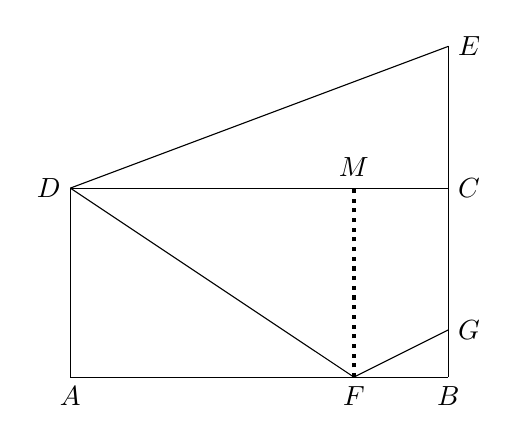
\begin{tikzpicture}[xscale=1.2,yscale=0.6]
		\coordinate (A) at (0,0);
		\coordinate (F) at (3,0);
		\coordinate (B) at (4,0);
		\coordinate (G) at (4,1);
		\coordinate (C) at (4,4);
		\coordinate (E) at (4,7);
		\coordinate (D) at (0,4);
		\draw (A) node[below] {$A$}--(F) node[below] {$F$};
		\draw (F)--(B) node[below] {$B$};
		\draw (B)--(G) node[right] {$G$};
		\draw (G)--(C) node[right] {$C$};
		\draw (C)--(E) node[right] {$E$};
		\draw (E)--(D) node[left] {$D$};
		\draw (D)--(A);
		\draw (D)--(C);
		\draw (D)--(F);
		\draw (F)--(G);
		% added
		\coordinate (M) at (3,4);
		\draw[dotted,line width=1.5pt] (F)--(M) node[above] {$M$};
	\end{tikzpicture}
	\end{center}
	}

	作$FM$,垂直相交于$CD$。因$\triangle{ADC}$面积为$90$,所以长方形$AFMD$面积为$2\times90=180$。由此,可得
	\[ \begin{aligned}
		S(\rectangle AFMD) : S(\rectangle ABCD) &= 180 : 240 \\
		\overline{AD}\cdot\overline{AF} : \overline{AD}\cdot\overline{AB} &= 3 : 4 \\
		\overline{FB} : \overline{AB} = 1 : 4 \ \mbox{。}
		\end{aligned} \ \mbox{。}
	\]

	另,由于$DE\parallel FG$,且$\triangle{BGF}$和$\triangle{CED}$皆为直角三角形,因此这两个三角形所有内角相等,即互为相似三角形。由此可得,
	\[ \begin{aligned}
			\overline{FB}:\overline{DC} &= \overline{BG} : \overline{CE} \\
			\overline{FB}:\overline{AB} &= \overline{BG} : \overline{CG} \\
			\overline{BG}:\overline{CG} &= 1 : 4 \\
			\overline{BG}:\overline{BC} &= 1 : 5 \ \mbox{。}
		\end{aligned}
	\]

	最后,我们得到
	\[ \begin{aligned}
			S(\triangle{BGF})
			&= \frac{1}{2}\overline{FB}\cdot\overline{BG} \\
			&= \frac{1}{2}\left(\frac{1}{4}\overline{AB}\right)\left(\frac{1}{5}\overline{BC}\right) \\
			&= \frac{1}{40}S(\rectangle ABCD) \\
			&= 6 \ \mbox{。}
		\end{aligned}
	\]
	\Qed
	\vspace*{30pt}

	\noindent 点评:
	\begin{enumerate}[label=(\alph*)]
		\item 几何题求面积,一般上有两种手段,一种是尽可能计算出边长的值,第二种是通过各种比例。前者一般需要更多的已知条件,后者则能避免前者的局限。
	\end{enumerate}

\end{document}
